%%%%%%%%%%%%%%%%%%%%%%%%%%%%%%%%%%%%%%%%%%%%%%%%%%%%%%%%%%%%%%%%%%%%%%%%%%%%%%%
%%                                                                           %%
%%   Stefanos Stefanou    													 %%
%%   ID : 27020363                                                           %%
%%   Department of Computer Science                                          %% 
%%   University of Reading, UK                                               %%
%%                                                                           %%
%%%%%%%%%%%%%%%%%%%%%%%%%%%%%%%%%%%%%%%%%%%%%%%%%%%%%%%%%%%%%%%%%%%%%%%%%%%%%%%
%%----------------------------------------------------------------------------------
% DO NOT Change this is the required setting A4 page, 11pt, onside print, book style
%%----------------------------------------------------------------------------------
\documentclass[a4paper,11pt,oneside]{book} 

%%-------------------------------------
%% Page margin settings - % half inch margin all sides (recommended)
%%-------------------------------------
\usepackage[margin=1.2in]{geometry} 

%%-------------------------------------
%% Font settings - % CM San or Arial (recommended)
%%-------------------------------------
% Switch the following two line off: to revert back to defult LaTex font (NOT recomended)
\usepackage{amsfonts}
\renewcommand*\familydefault{\sfdefault}


%%-------------------------------------
%% Diagrams
%%-------------------------------------
\usepackage{tikz}


%%-------------------------------------
%% Math/Defination/Theorem/Algorithm packages settings 
%%-------------------------------------
\usepackage[cmex10]{amsmath}
\usepackage{amssymb}
\usepackage{amsthm}
\newtheorem{mydef}{Definition}
\newtheorem{mytherm}{Theorem}

%%-------------------------------------
%% Algorithms/Code Listing environment settings  - 
%% Please do not change these settings
%%-------------------------------------
\usepackage{algorithm}
\usepackage{algpseudocode}
\renewcommand{\algorithmicrequire}{\textbf{Input:}}
\renewcommand{\algorithmicensure}{\textbf{Output:}}
\usepackage[utf8]{inputenc}
\usepackage{listings}
\usepackage{xcolor}
\definecolor{codegreen}{rgb}{0,0.6,0.1}
\definecolor{codegray}{rgb}{0.5,0.5,0.5}
\definecolor{codeblue}{rgb}{0.10,0.00,1.00}
\definecolor{codepurple}{rgb}{0.58,0,0.82}
\definecolor{backcolour}{rgb}{1.0,1.0,1.0}
\lstdefinestyle{mystyle}{
    backgroundcolor=\color{backcolour},   
    commentstyle=\color{codegreen},
    keywordstyle=\color{codeblue},
    numberstyle=\tiny\color{codegray},
    stringstyle=\color{codepurple},
    basicstyle=\ttfamily\footnotesize,
    breakatwhitespace=false,         
    breaklines=true,                 
    captionpos=b,                        
    keepspaces=true,                 
    numbers=left,                    
    numbersep=5pt,                  
    showspaces=false,                
    showstringspaces=false,
    showtabs=false,                  
    tabsize=2,
    frame=none
}
\lstset{style=mystyle}

%%-------------------------------------
%% Graphics/Figures environment settings
%%-------------------------------------
\usepackage{graphicx}
\usepackage{subfigure}
\usepackage{caption}
\usepackage{lipsum}

%%-------------------------------------
%% Table environment settings
%%-------------------------------------
\usepackage{multirow}
\usepackage{rotating}
\usepackage{makecell}
\usepackage{booktabs}
%\usepackage{longtable,booktabs}

%%-------------------------------------
%% List of Abbreviations settings
%%-------------------------------------
\usepackage{enumitem}
\newlist{abbrv}{itemize}{1}
\setlist[abbrv,1]{label=,labelwidth=1in,align=parleft,itemsep=0.1\baselineskip,leftmargin=!}

%%-------------------------------------
%% bibliography/Refernces settings   - Harvard Style was used in this report
%%-------------------------------------
\usepackage[hidelinks]{hyperref}
\usepackage[comma,authoryear]{natbib}
\renewcommand{\bibname}{References} % DO NOT remove or switch of 

%%-------------------------------------
%% Appendix settings     
%%-------------------------------------
\usepackage[toc]{appendix}
%%%%%%%%%%%%%%%%%%%%%%%%%%%%%
%%%%     SETTING ENDS  %%%%%%
%%%%%%%%%%%%%%%%%%%%%%%%%%%%%
\begin{document}

    \captionsetup[figure]{margin=1.5cm,font=small,name={Figure},labelsep=colon}
    \captionsetup[table]{margin=1.5cm,font=small,name={Table},labelsep=colon}
    \setlipsumdefault{1}
    
    \frontmatter
          
    \begin{titlepage}      
        \begin{center}
            
\includegraphics[width=3cm]{figures/uorlogo.png}\\[0.5cm]
            {\LARGE University of Reading\\[0.5cm]
                Department of Computer Science}\\[2cm]
            %{\color{blue} \rule{\textwidth}{1pt}}
            
            % -------------------------------
            % You need to edit some details here
            % -------------------------------  
            
            %------------------------------  An AI-assisted decision making system for thyroid nodule classification ----------------------------------%
            % chnage the following line
            \linespread{1.2}\huge {An AI-assisted decision making system for thyroid nodule classification}
            
            
            \linespread{1}~\\[2cm]
            %{\color{blue} \rule{\textwidth}{1pt}}
            
            %------------------------------  Your Name  -------------------------------%
            {\Large Stefanos Stefanou}\\[1cm] 
            
            %-------------------------- Your Superviosr's name(s) ---------------------%
            % chnage the following line
            {\large \emph{Supervisor:} Huizhi Liang}\\[1cm] % if applicable
            
            % PLEASE DO NOT CHANGE THIS TEXT %
            \large A report submitted in partial fulfilment of the requirements of\\the University of Reading for the degree of\\ Bachelor of Science in \textit{Computer Science}\\[0.3cm] 
            \vfill
            
            
            April, 2021% Please update this date you can use \date{April 2020} for fixed date
        \end{center}
    \end{titlepage}

    % -------------------------------------------------------------------
    % Declaration
    % -------------------------------------------------------------------
    \newpage
    \thispagestyle{empty}
    \chapter*{\Large Declaration}
    % PLEASE CHANGE THIS TEXT EXCEPT YOUR NAME%
    % -------------------------------
    % PLEASE ONLY UPDATE HERE -- PLEASE WRITE YOUR NAME %    
    % ------------------------------- 
    I, Stefanos Stefanou, of the Department of Computer Science, University of Reading, confirm that all the sentences, figures, tables, equations, code snippets, artworks, and illustrations in this report are original and have not been taken from any other person's work, except where the works of others have been explicitly acknowledged, quoted, and referenced. I understand that if failing to do so will be considered a case of plagiarism. Plagiarism is a form of academic misconduct and will be penalised accordingly.\\[1cm]
    
    
    \begin{flushright}
        %------------------------------ PLEASE UPDATE  Your Name  -------------------------------%
        % change the following line
        Stefanos Stefanou % Please change it to your name
        
        April, 2021
    \end{flushright}
     
    % -------------------------------------------------------------------
    % Abstract and Acknowledgement
    % -------------------------------------------------------------------
    
    \chapter{Abstract}
\label{abstract}

Deep learning has found numerous applications in the health care community. Recently, a massive explosion of research on the relevant field, 
driven by large amounts of available data, has generated important disease prevention and identification results. Fine Needle Aspiration (FNA) 
is the dominant procedure for thyroid nodule classification. FNA has associated risks and expenses, and in this project,
we will try to reduce both using the recent advancements in Artificial Intelligence and Deep Learning. Our primary goal is to 
bring closer the radiologists 'on the field' with those complex algorithms and provide value to real patients by providing an interface, 
in the form of a web application, for probabilistically predicting the severity and the category of a given module.

    % -------------------------------------------------------------------
	% Acknowledgement
	% -------------------------------------------------------------------
   
    %\chapter*{\center \Large  Acknowledgments}

Acknowledgments section is optional. You may like to acknowledge the support and help of your supervisor(s), friend(s), or any other person(s), department(s), institute(s).


    
    % -------------------------------------------------------------------
    % Contents, list of figures, list of tables
    % -------------------------------------------------------------------
    
    \tableofcontents
    %\listoffigures
    %\listoftables
    
    % -------------------------------------------------------------------
    % Main chapters and sections of your Project
    % Everything from here on your words and works 
    % -------------------------------------------------------------------
    \mainmatter
    % Read for preparation of document in LaTex 
    % Lamport, L. (1986), LATEX: A Document Preparation System, Addison-Wesley.
    
    
    \chapter*{\center \Large  Acknowledgments}

Acknowledgments section is optional. You may like to acknowledge the support and help of your supervisor(s), friend(s), or any other person(s), department(s), institute(s).


    \chapter{Introduction}
\label{1}

Deep learning has found numerous applications in the health care community. Recently, a massive explosion of research on the relevant field, 
driven by large amounts of available data, has generated important disease prevention and identification results. Fine Needle Aspiration (FNA) 
is the dominant procedure for thyroid nodule classification. FNA has associated risks and expenses, and in this project,
we will try to reduce both using the recent advancements in Artificial Intelligence and Deep Learning. Our primary goal is to 
bring closer the radiologists 'on the field' with those complex algorithms and provide value to real patients by providing an interface, 
in the form of a web application, for probabilistically predicting the severity and the category of a given module.

\subsubsection{Abbreviations}FNA(Fine Needle Aspiration), AI(Artificial Intelligence), DP(Deep Learning)Abbreviations 
\subsubsection{Keywords}FNA(Fine Needle Aspiration), AI(Artificial Intelligence), DP(Deep Learning)Abbreviations 



    \chapter{Literature Review}
	\section{Brief Table of books}
	\begin{table}[H]
		\begin{tabular}{lllll}
			ISBN 			& Name 	& Type  &  &  \\
			N/A  			&ST1PS-18-9A: Probability and Statistics (2018/19)&Module Lectures&  &  \\
			9780030105678  	&Linear Algebra and Its Applications&Book&  &  \\
			9780131687288  	&Digital Image Processing&Book&  &  \\
			9780262035613  	&Deep Learning &Book&  &  \\
			9780128104088  	&Deep Learning for Medical Image Analysis&Book&  &  \\
			9781491962244  	&Hands-on machine learning with scikit-learn and tensorflow&Book&  &  \\
		\end{tabular}
	\end{table}
	\section{Brief Table of papers}
	\begin{itemize}
		\item Ye, H., Hang, J., Chen, X. et al. An intelligent platform for ultrasound diagnosis of thyroid nodules. Sci Rep 10, 13223 (2020). https://doi.org/10.1038/s41598-020-70159-y
		\item Nguyen DT, Pham TD, Batchuluun G, Yoon HS, Park KR. Artificial Intelligence-Based Thyroid Nodule Classification Using Information from Spatial and Frequency Domains. J Clin Med. 2019;8(11):1976. Published 2019 Nov 14. doi:10.3390/jcm8111976
		\item Manivannan T, Ayyappan N. Classification of thyroid nodules using ultrasound images. Bioinformation. 2020;16(2):145-148. Published 2020 Feb 29. doi:10.6026/97320630016145
		\item Nguyen DT, Kang JK, Pham TD, Batchuluun G, Park KR. Ultrasound Image-Based Diagnosis of Malignant Thyroid Nodule Using Artificial Intelligence. Sensors (Basel). 2020;20(7):1822. Published 2020 Mar 25. doi:10.3390/s20071822
		\item Chen J, You H, Li K. A review of thyroid gland segmentation and thyroid nodule segmentation methods for medical ultrasound images. Comput Methods Programs Biomed. 2020 Mar;185:105329. doi: 10.1016/j.cmpb.2020.105329. Epub 2020 Jan 9. PMID: 31955006.
	\end{itemize}
	\section{Analytic Report: Books}
	\subsection{Learning Path Visualised}
	The reader should note that many of the learning nodes for the following diagram already existed in the student's program in parts 1 and 2. The reference here is sorely for pointing out the need for a complete revision over the aforementioned topics and for clarity.
	\begin{figure}[H]
		\iftrue
		\caption{Learning Path}
		\centering
		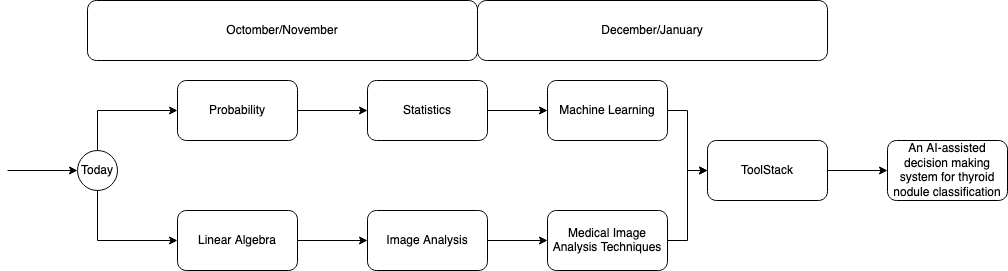
\includegraphics[scale=0.3]{figures/path}
		\fi
	\end{figure}
	\subsection{(Probability/Statistics)ST1PS-18-9A: Probability and Statistics (2018/19)}
	In part 1, my module \textit{Probability and statistics} covers everything essential regarding my statictical background for this project.
	\subsection{(Linear Algebra)Linear Algebra and Its Applications}
	This excellent book will supplement my knowledge of linear algebra, covers almost anything that I will need later in the image analysis part.
	\subsection{(Image Analysis)Digital Image Processing Author(s): Rafael C. Gonzalez, Richard E. Woods + CS3IA16-20-1A: Image Analysis (2020/21)}
	This book, recommended by the lecturer in CS3IA16, will supplement my knowledge in image analysis and basic image transformation algorithms needed for the preprocessing part of the Machine learning service. 
	\subsection{(Machine Learning)Deep Learning Book by Aaron Courville, Ian Goodfellow, and Yoshua Bengio}
	This excellent book is an introduction to Machine learning with Deep Learning techniques, much needed in the AI-analy
	\subsection{(Techniques)Deep Learning for Medical Image Analysis}
	This book has plenty of industry-standard techniques for medical image analysis. It will help me catch up with the latest research methods in this field.
	\subsection{(ToolStack)Hands-On Machine Learning with Scikit-Learn and TensorFlow: }
	This book will teach me the basic AI-toolkit stack, as well as the practical techniques for writing intelligent systems.
	\subsection{Papers}
	Around that time, i will start learning specialized techiques for this domain. The aforementioned papers will be my source of information.	

    \chapter{Requirement Analysis}
	
	\section{Introduction}
		Before we even start exploring this project and its features, it is important to strictly define the requirements need to be fulfilled and the
		scope of this project. failing to perform an requirement analysis beforehand puts additional and unsessesary risks to the project due to the
		varying scope and target set.


    \chapter{Entity Relation Analysis}
	\section{Introduction}
	After the requirements have been set. We need to translate them into workable relational entities in order to be able to modeled through a classical
	relational database system (RDBMS).
	\section{Entities}
	We will start our exploration by defining our entities for this project.
	\subsection{Scan}
	A scan is the result of an ultrasound scan performed in a specific patient(see [\ref{patient-definition})]. A scan entity has certain attributes
	\begin{center}
		\begin{tabular}{ |c|c| } 
			\hline
			Image & The image produced by the ultrasound scan. 360x560 pixels\\
			Prediction & The result of the prediction algorithm. Acceptable Values = {Maligrant, Benign}  \\
			Results & The logs of the algorithm performed the prediction, Optional \\
			Algorithm & The algorithm used to perform the prediction. Acceptable Values = {SVC,RES} \\
			Token& The scan identifier across the application services. token type is UUID [\cite{rfc4122}] \\
			\hline
		\end{tabular}
	\end{center}
	\subsection{Patient}
	\label{patient-definition}
	A patient is a physical person that is suspected to have a thuroid nodule. A person may have 0 up to n scans, where n is the theoretical
	maximum number of records(no limit is enforced by the database or the application). A patient has characteristics explaned below
	\begin{center}
		\begin{tabular}{ |c|c| } 
			\hline
			First Name & The first name of the patient.\\
			Last Name & The last name of the patient \\
			NiNo & The National Insurance Number(NiNo) of the patient \\
			Enrolled Date & The Date that the patient was registered in the system \\
			Ascosiate Doctor& The Doctor identification number, handling the case of the patient(see \ref{doctor-definition}) \\
			Comments& The Doctors(see \ref{doctor-definition}) comments for the particular patient\\
			\hline
		\end{tabular}
	\end{center}
	\subsection{Doctor}
	\label{doctor-definition}
	A doctor is a physical person with access on the system. Is the end-user of the system and has rights of uploading ultrasound image
	scans and retrieve predictions for those scans. It can also provide feedback to the system for a given prediction to be used for 
	further research and develepoment. A doctor has specific characteristics presented below.
	\begin{center}
		\begin{tabular}{ |c|c| } 
			\hline
			Username & Plain-text username\\
			Password & MD5 Hashed[\cite{rfc1321}] and salted[\cite{MANBER1996171}] password \\
			First Name & National Insurance Number[\cite{nino-format}] \\
			Last Name & The date that the patient was registered in the system \\
			Title& The title of the doctor.\\
			Enrolled Date& The date and time of the user enrolled to the system\\
			Last Seen& The date and time of last login of the user \\
			Online Status& The status of the user, acceptable values are Connected,Not Connected \\
			Tasks& The number of scans uploaded by the user \\
			\hline
		\end{tabular}
	\end{center}
	\subsection{Notification}
	\label{notification-definition}
	A notification is a short message from the system to the end-user(The doctor). Its sole purpose is to inform the user about
	various events that may interest the end-user. An example of this may be that the scan results for a given scan task are ready 
	to view. A notification has specific characteristics witch are displayed and explained below.
	\begin{center}
		\begin{tabular}{ |c|c| } 
			\hline
			Message & The message in question\\
			Ascosiated Doctor & The receipient doctor identification number \\
			Created Date & The Date and Time where the event in question where happened\\
			\hline
		\end{tabular}
	\end{center}
	\section{Entity Relations}
	The aforementioned entities have well defined relations. An exhaustive list is given below
	\begin{itemize}
		\item A doctor has many patients (1 - $\infty$)
		\item A doctor has many notifications(1 - $\infty$)
		\item A Patient has many Scans(1 - $\infty$)
	\end{itemize}
	A above relations can be summarized in the following E-R\footnote{Entity-Relation} Diagram
	\begin{figure}[H]
		\iftrue
		\centering
		\caption{Entity-Relation Diagram}
		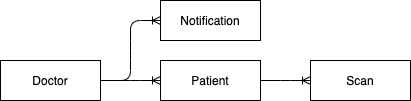
\includegraphics[scale=0.5]{figures/Entity-Relation-Fig}
		\fi
	\end{figure}



    \chapter{Users Perspective}
\label{users_perspective}
	\section{Introduction}
		In this section, we will start our exploration of the application and its features. As the nature of the requirements of this
		the system is complicated. Unavoidably the system will be complex as well. Taking this into consideration, we will follow a natural top-to-bottom
		approach explaining its internals, starting as end-users and seeing the system as a black box. In this section, we will analyze its 
		functionality from the user's perspective. This section may also serve as an instruction manual for the end-user as it contains everything needed
		for an inexperienced user to start working with the software.
	\section{Login and Authentication}
		\begin{figure}[H]
			\iftrue
			\centering
			\caption{Login Screen}
			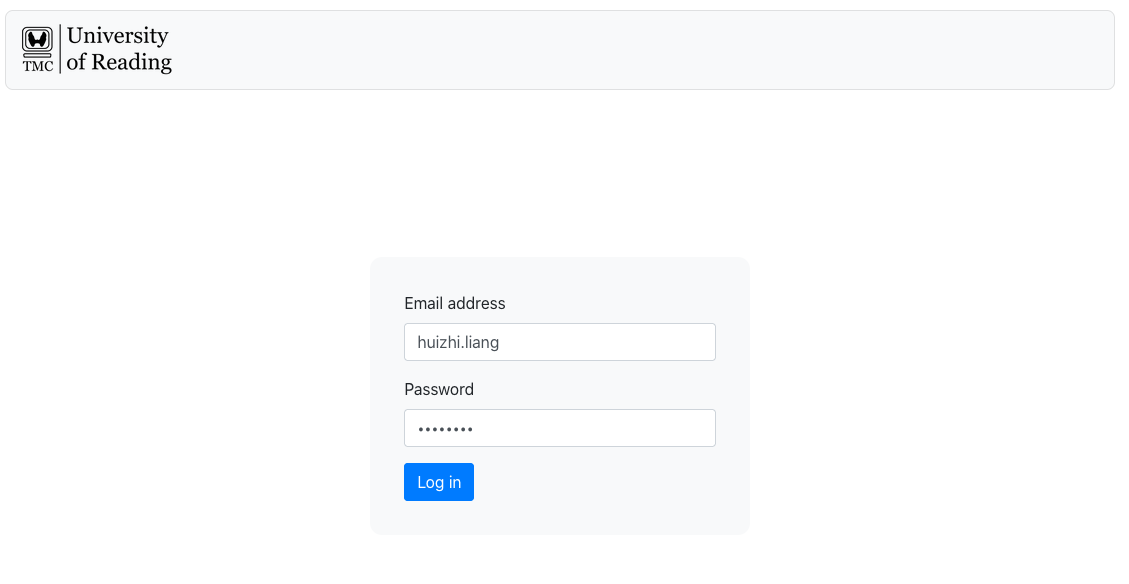
\includegraphics[scale=0.3]{figures/login}
			\fi
		\end{figure}
		The login screen is the first screen that our end-users will encounter. Here a username and a password is required to be given by the 
		user to log in. The Credentials of the user remain encrypted during the process of login, as the system utilizes an HTTPS[\cite{rfc2818}] 
		protocol for its connection, this is essential for the first non-functional requirement about security (see \ref{non-functional-requirements}).
		The username and the password may be requested by the system administrator or the NOC\footnote{Network Operations Center} of the hospital.
	\section{Home}
		\begin{figure}[H]
			\iftrue
			\centering
			\caption{Home Screen}
			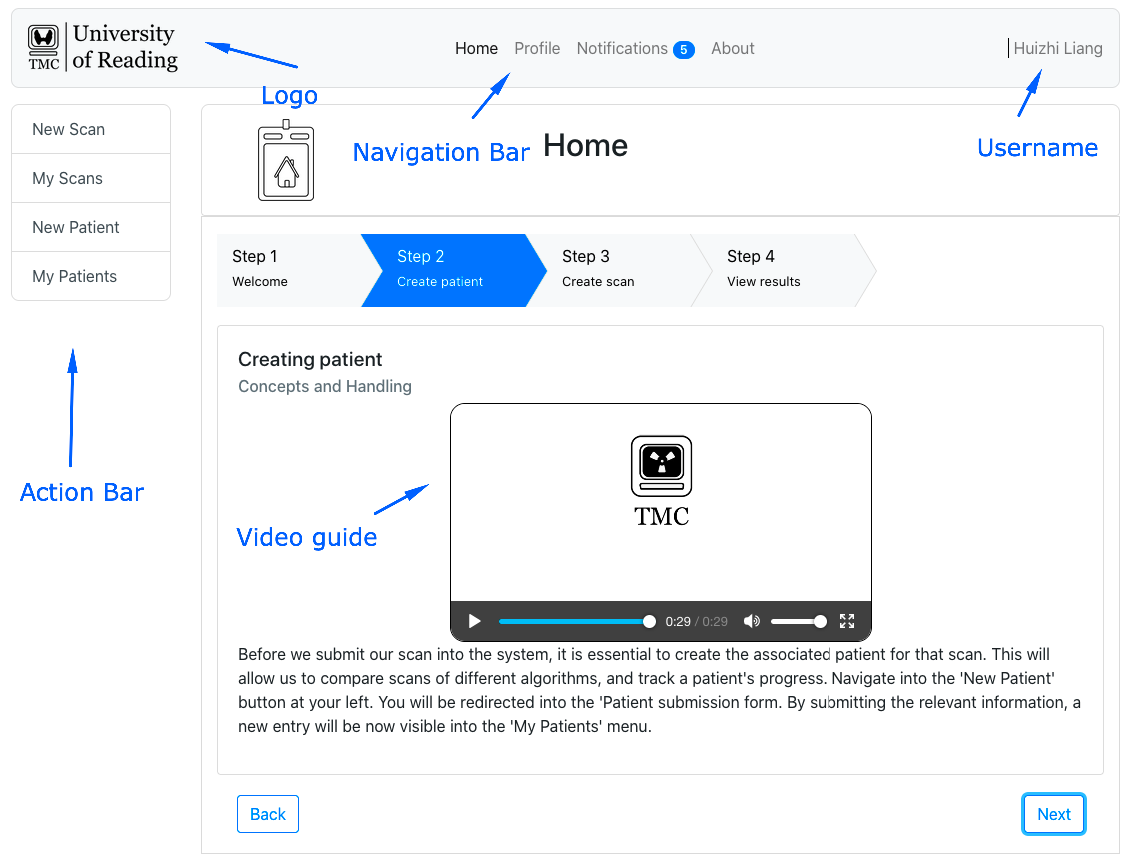
\includegraphics[scale=0.3]{figures/home}
			\fi
		\end{figure}
		After the login process is completed. The user encounters the 'home screen. From here, it is possible to navigate to the features of the software
		as well as learn about how the software can be utilized through detailed guides and videos. The UI/UX\footnote{User Interface-User Expieriance} 
		has been designed to be as user-friendly as possible. Some areas of interest are given below.
		\begin{center}
			\begin{tabular}{ |c|c| } 
				\hline
				Action bar & The Actions that can be performed using the software can be accesed from here.\\
				Navigation bar & General information and notification bar. \\
				\hline
			\end{tabular}
		\end{center}
	\section{Navigation bar}
		In this section, we will briefly look at the options under the Navigation bar.
		\subsection{Profile}
			\begin{figure}[H]
				\iftrue
				\centering
				\caption{Profile}
				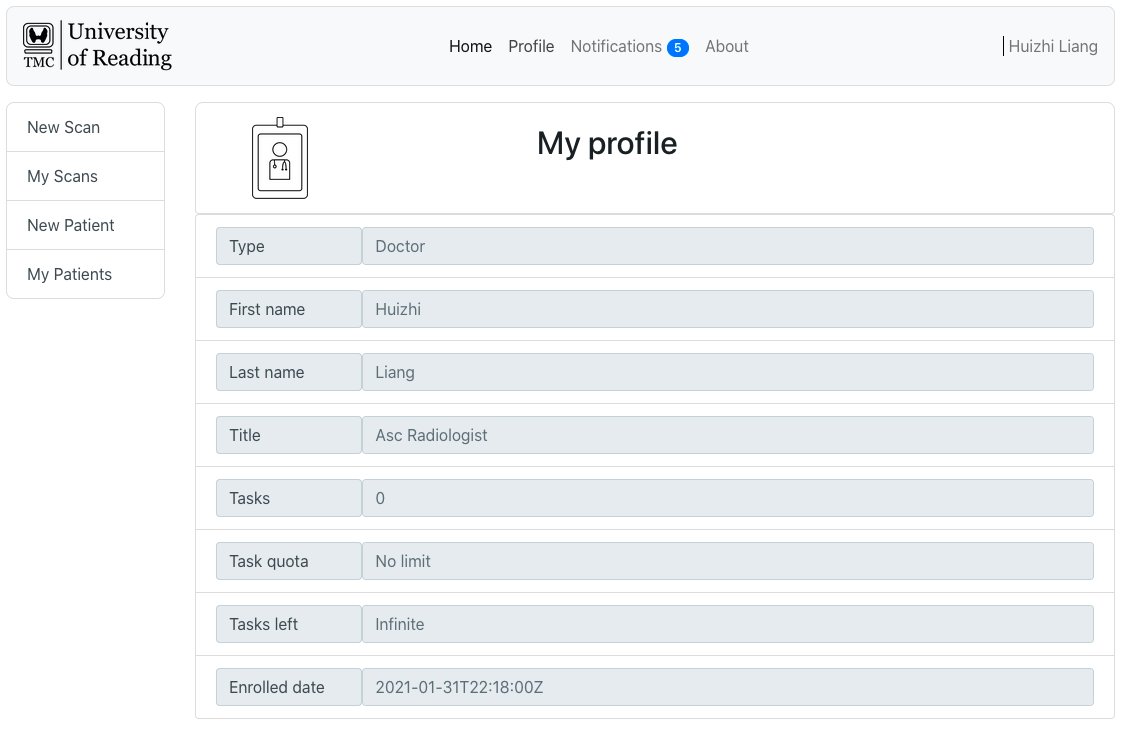
\includegraphics[scale=0.3]{figures/profile}
				\fi
			\end{figure}
			In the profile section, the user can see its associated information, saved on the registration date. 
			The information for security reasons cannot be altered by the user itself, but only after a request to 
			the system administrator or NOC\footnote{Network Operations Center}.
		\subsection{Notifications}
			\begin{figure}[H]
				\iftrue
				\centering
				\caption{Notifications}
				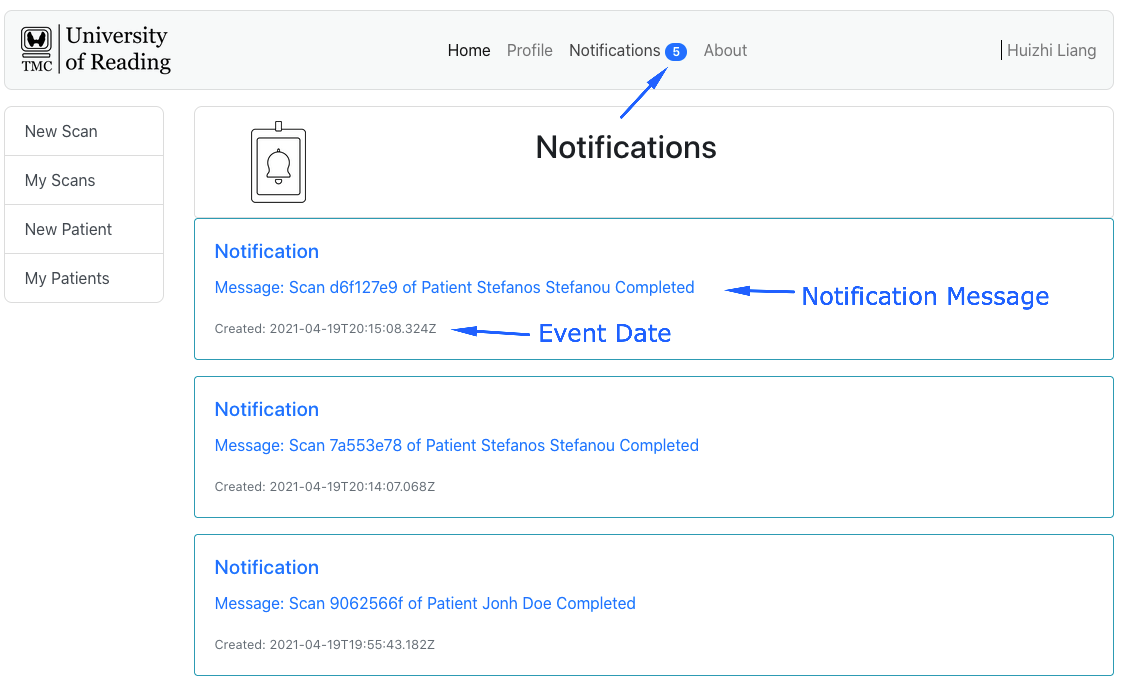
\includegraphics[scale=0.3]{figures/notifications}
				\fi
			\end{figure}
			In the notification section, helpful information about events that may interest the end-user can be found, 
			such as the fact that uploaded scan results are ready to view. 
		\subsection{About}
			\begin{figure}[H]
				\iftrue
				\centering
				\caption{About}
				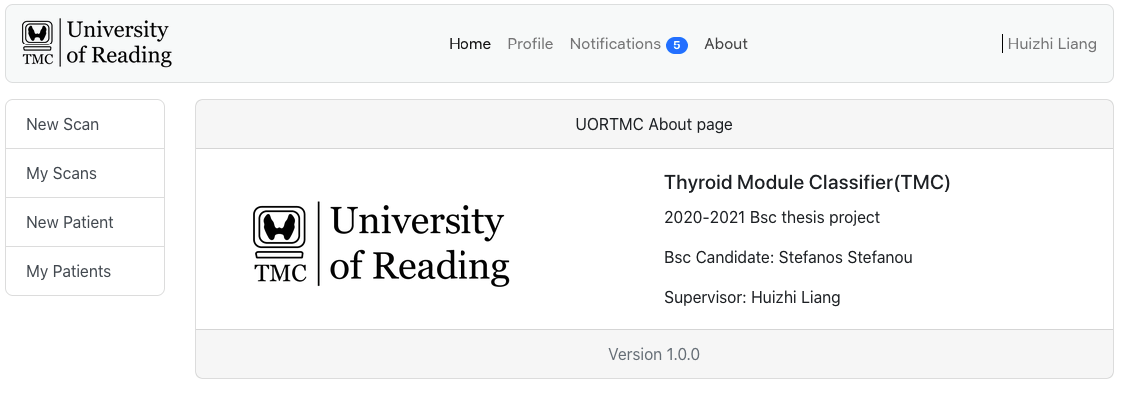
\includegraphics[scale=0.3]{figures/about}
				\fi
			\end{figure}
			From here, a user may found helpful information about the software, such as the current version.
	\section{Action Bar}
		In this section, we will briefly look at the options under the Action Bar.
		\subsection{My Patients}
			\begin{figure}[H]
				\iftrue
				\centering
				\caption{Patients List}
				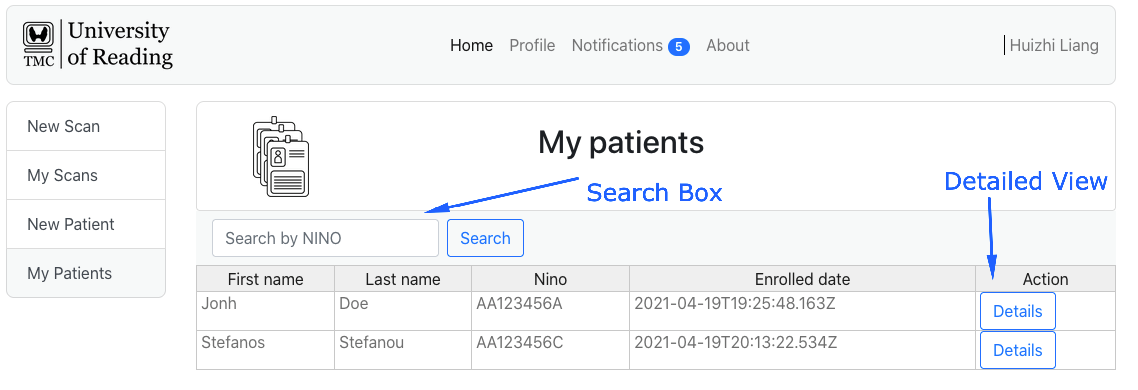
\includegraphics[scale=0.3]{figures/mypatients}
				\fi
			\end{figure}
			This page will show us a list of the currently registered patients. Each end-user(doctor) may only see its 
			patients and not others. The end-user can search the list based on NiNo[\cite{nino-format}] of the given 
			patient for convenience. The end-user can also view the details of a given patient and record various 
			notes/comments for that patient by clicking the 'Details' button on his selected patient, as seen below. 
			Finally, clicking the button 'View Scans' can see the specific patient history of uploaded scans.
			\begin{figure}[H]
				\iftrue
				\centering
				\caption{Patient Details}
				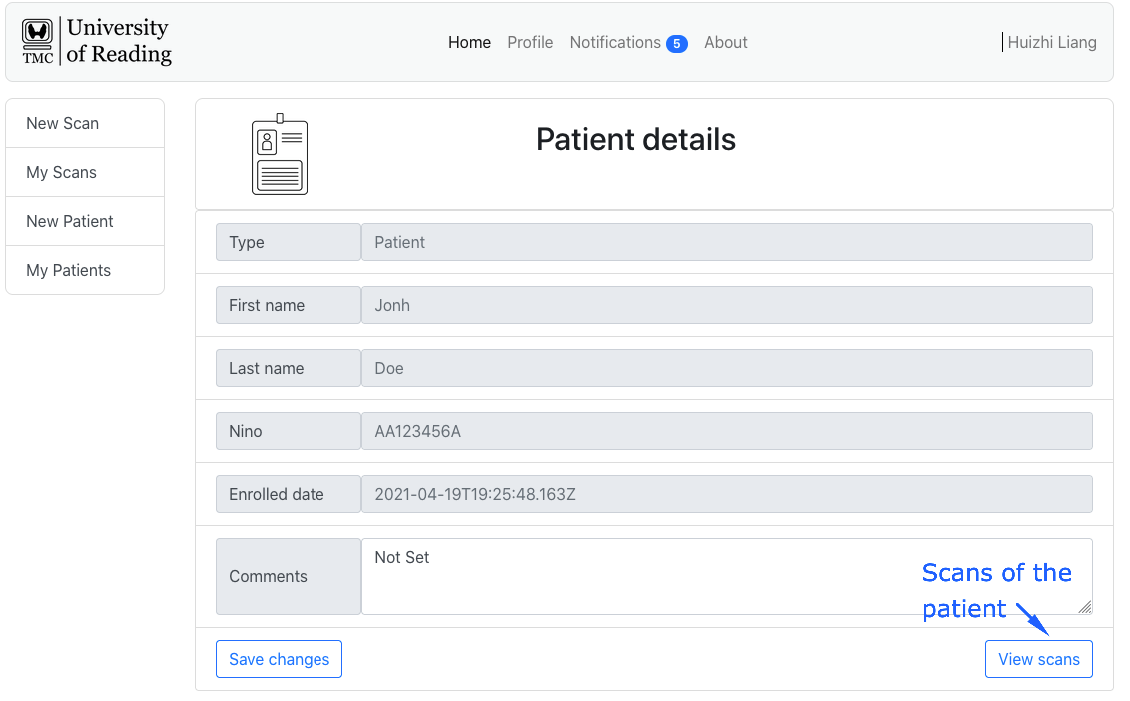
\includegraphics[scale=0.3]{figures/mypatients2}
				\fi
			\end{figure}
		\subsection{New Patient}
			\begin{figure}[H]
				\iftrue
				\centering
				\caption{New Patient}
				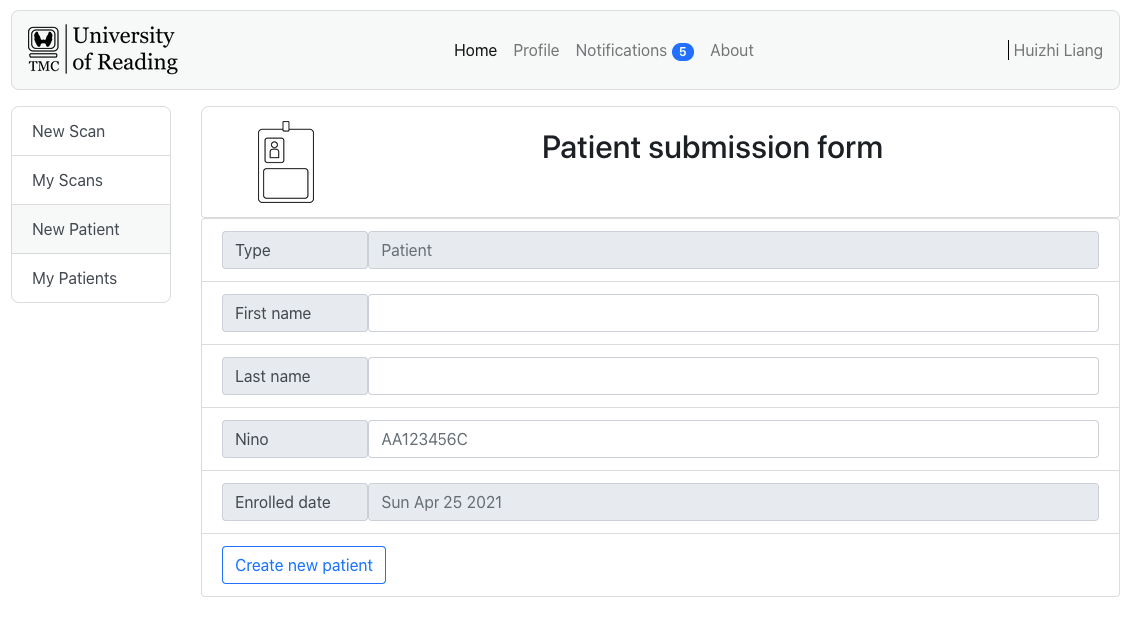
\includegraphics[scale=0.3]{figures/newpatient}
				\fi
			\end{figure}
			By clicking the 'New Patient' action on Action Bar, the user can register a new patient on the system. The following conditions need to 
			be met for the operation to be successful.
			\begin{itemize}
				\item First name length should be more than 2 characters, encoded as UTF-8[\cite{rfc3629}]
				\item Last name length should be more than 2 characters, encoded as UTF-8[\cite{rfc3629}]
				\item NiNo should be at standard format [\cite{nino-format}], encoded as UTF-8[\cite{rfc3629}]
			\end{itemize}
			Failing to fulfill these constraints should lead to an error, as shown below.
			\begin{figure}[H]
				\iftrue
				\centering
					\caption{New Patient Error}
				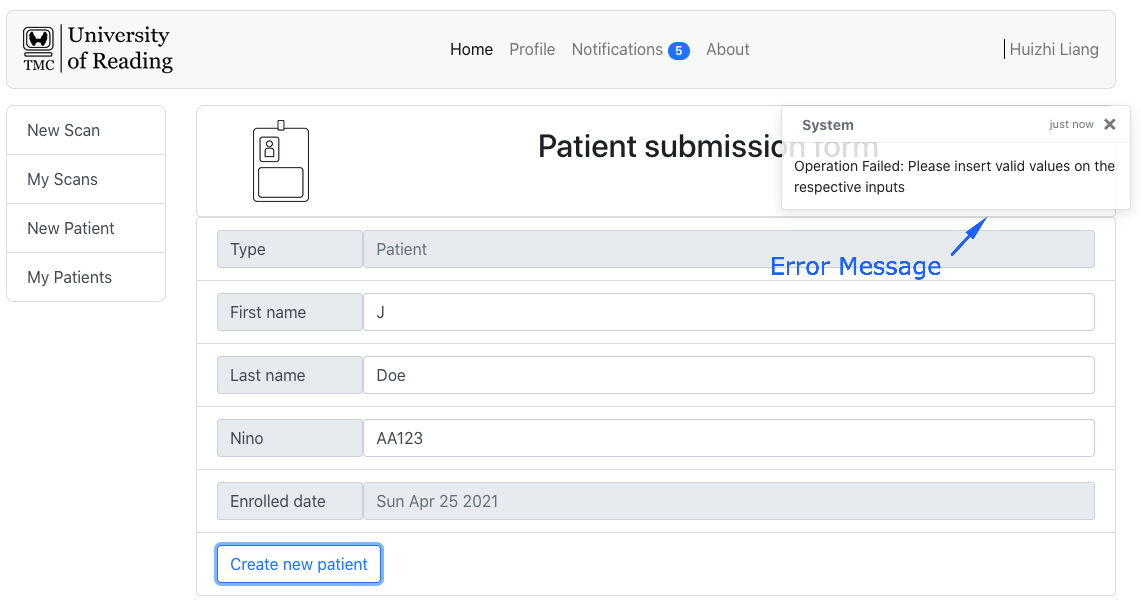
\includegraphics[scale=0.3]{figures/newpatient-error}
				\fi
			\end{figure}
		\subsection{My Scans}
			\begin{figure}[H]
				\iftrue
				\centering
				\caption{My Scans}
				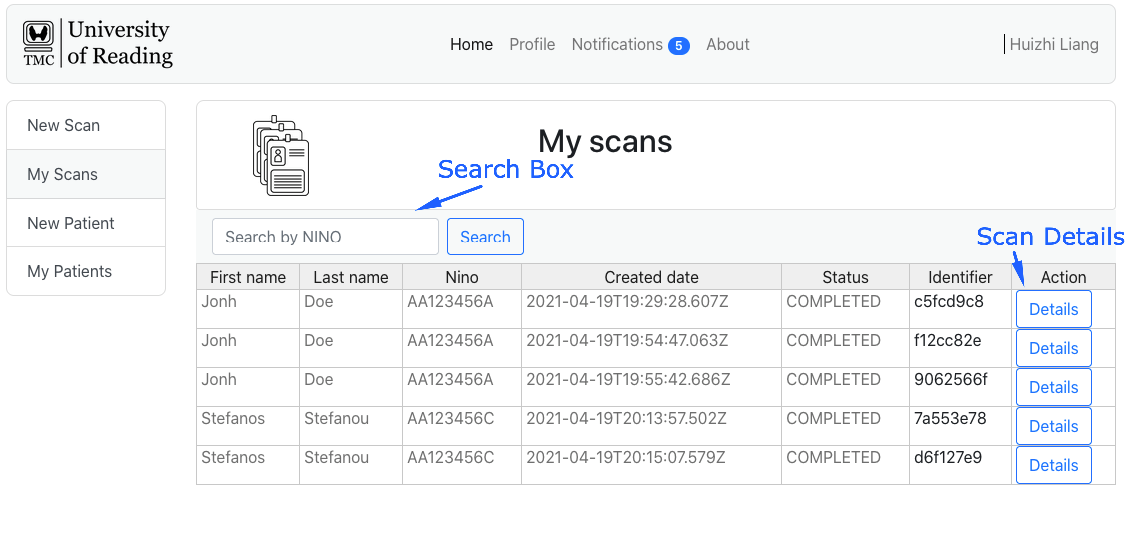
\includegraphics[scale=0.3]{figures/myscans}
				\fi
			\end{figure}
			'MyScans' are a complete list with all submitted scans for a given end-user. 
			The user can search for the scans of a specific patient by using the search box and viewing the 
			scan results (if a given scan is complete) by clicking the 'Details' button of the scan in question.
			\begin{figure}[H]
				\iftrue
				\centering
				\caption{Scan results}
				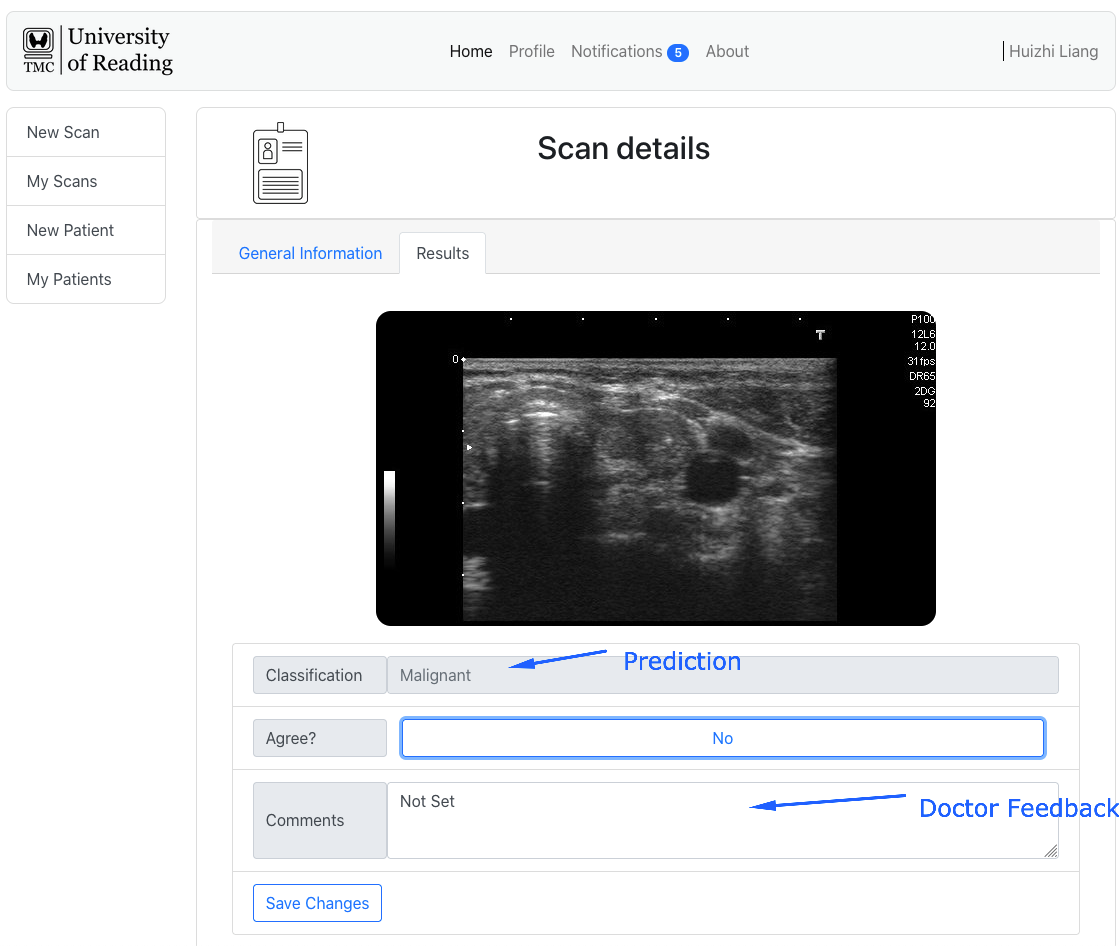
\includegraphics[scale=0.3]{figures/myscans-details}
				\fi
			\end{figure}
		\subsection{New Scan}
			\begin{figure}[H]
				\iftrue
				\centering
				\caption{New Scan}
				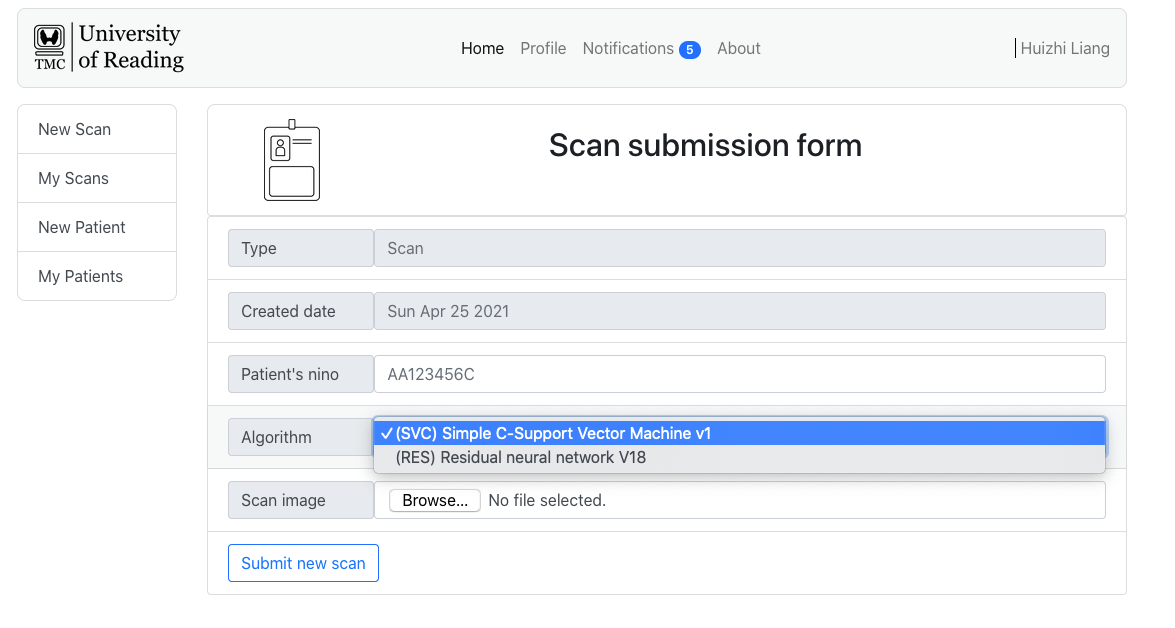
\includegraphics[scale=0.3]{figures/newscan}
				\fi
			\end{figure}
			By clicking the 'New Scan' action, the user is redirected into the scan submission form. Here it is possible to 
			submit a new ultrasound image for a given patient.The user can also select the algorithm for performing the 
			classification (see \ref{prediction-service}). The operation to be completed should meet the following criteria.
			\begin{itemize}
				\item Patients Nino should be in standard format[\cite{nino-format}] and encoded as UTF-8[\cite{rfc3629}]
				\item Scan Image should be a ISO/IEC 10918-1/JPEG[\cite{jpeg-iso10918-1}] format with 360x560 resolution. The image name
				should be encoded as UTF-8[\cite{rfc3629}]
			\end{itemize}
			Failing to fulfill these constraints should lead to an error, as shown below.
			\begin{figure}[H]
				\iftrue
				\centering
				\caption{Invalig image format (PNG) error}
				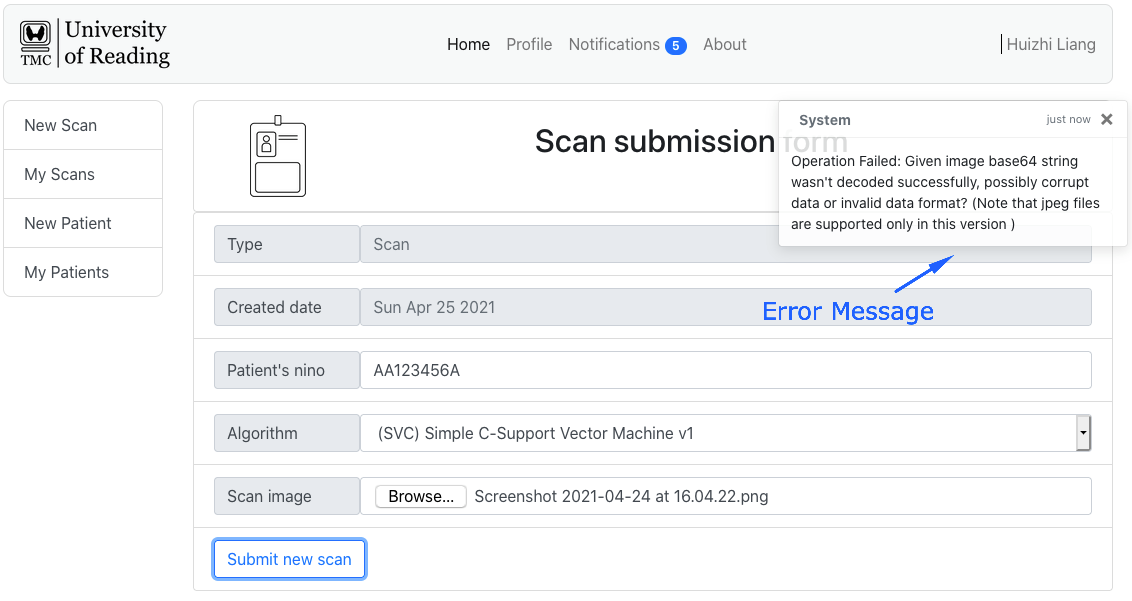
\includegraphics[scale=0.3]{figures/newscan-error}
				\fi
			\end{figure}
			
			
			
			
			
			
			
		
	




    \chapter{Abstracted View of the System}
	\label{4}
	In this chapter, we will introduce the architecture of our system, explaining the essential elements
	that is composed of, and their interactions.
	\begin{figure}[H]
		\iftrue
		\caption{Essential System Components}
		\centering
		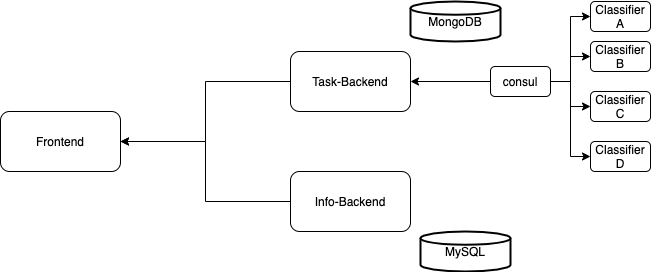
\includegraphics[scale=0.3]{figures/system-overview}
		\fi
	\end{figure}
	\section{Frontend Web App}
		The Frontend component has the responsibility of being the edge in our system.
		\begin{figure}[H]
			\iftrue
			\caption{Our system's edge}
			\centering
			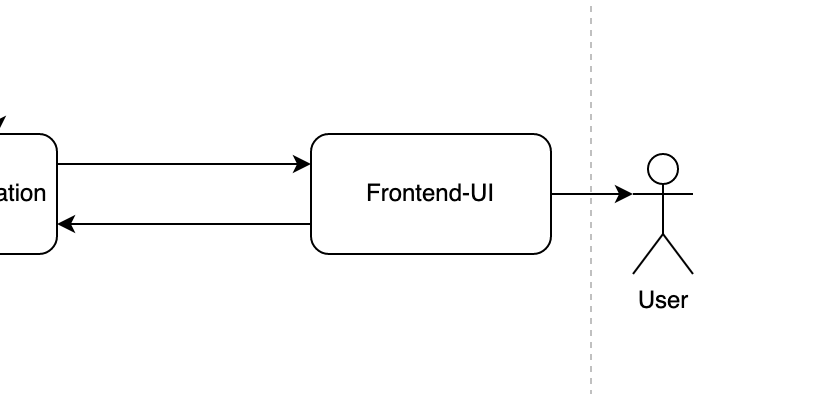
\includegraphics[scale=0.3]{figures/frontend-actor}
			\fi
		\end{figure}
		Every action from our users, should be channeled through the frontend.Our frontend is a web-based application, 
		and as an consequence of that, a design desision is that the API between the web app and the backend application
		will not be a public one. This desision will increase the security of our system, as the proccess of writing 
		spam bots will be significantly harder without a known API. More information about the API(Application 
		programming interface) will be given below.
	\section{Backend}
		There is a number of design choices that we have made on our Backend System, in order to increase security, and
		decrese complexity. Our Backend System follows the design principles of the microservice pattern. Microservice pattern
		tries to decrease complexity and increase safety by splitting the internal logic of a system into several components called
		'Microservices'. Each microservice is essentially a server that handles a small portion of the systems logic. As opposed to the
		monolithic services, microservices have a number of advantages such as
		\begin{itemize}
			\item Highly maintainable and testable
			\item Loosely coupled
			\item Independently deployable
			\item No Single Point of Failure
		\end{itemize}
		\subsection{Information Backend}
			The first of our services is the Information Backend. This service will have the responsibility to handle the information
			related to a scan, as well as its statistics and ascosiations between scans and patients. The majority of the models composing
			our systems will be available though this service, via a well designed API.
		\subsection{Task Backend}
			This microservice will have the responsibility to trigger prediction and classification tasks for our system. The whole procedure,
			due to its CPU Intensive nature, will have to be asyncronous and to be executed in the background. The Frontend will sent a request for
			a given task, and the server will have to return a token, ascosiated for that particular task. Later, The frontend may request to learn the
			progress of its task or its results(if completed) by using the relevant token. This design choice is unavoidable given that the HTTP protocol
			has embedded the notion of 'timeout', it is just impossible and impractical to wait untill a given task is complete. Another great advantage of 
			this asyncronous design is the fact that multiple users may request Tasks without eliminating the server's resources, such as CPU time and amount of
			RAM available. Indepedent of the number of requests, the server will implement a queue FIFO (First-In-First-Out) strategy and it will inform its users
			when the task is ready to be seen. 
		\subsection{Classification Backend}
			By using multiple classification techniques, our system will reduce the probability of an false prediction further. So one of our 
		
		
		
				
					
			
		
	

    \chapter{The Frontend}
\label{ch:lit_rev}
\subsection{Technology Stack}
In the construction of our system, we will need a number of open source technologies, libraries and standards to support our
develepoment. An exhaustive list is given below
\begin{itemize}
	\item HTML5
	\item CSS3
	\item Javascript
	\item React.Js
	\item Boostrap
\end{itemize}
\subsubsection{HTML5}
HTML5 is a markup language mainly used for structuring content on 
the World Wide Web. The its last major version(version 5.0) it is recommended
by the World Wide Web Consortium (W3C). The responsible organisation WHATWG 
(Web Hypertext Application Technology Working Group) is a consortium of the 
major browser vendors(Apple, Google, Mozilla, and Microsoft)\cite{gudeliauskas_2019}.
\subsubsection{CSS3}
CSS stands for Cascading Style Sheets with an emphasis placed on “Style.” 
While HTML is used to structure a web document, CSS comes through and 
specifies your document’s style—page layouts, colors, and fonts are all 
determined with CSS\cite{morris_2020}. We will use CSS, version 3, to make our frontend
application aesthecaly pleasing and easy-to-use for our end-users.
\subsubsection{Javascript}
longside HTML and CSS, JavaScript is one of the major technologies of the World Wide Web.
JavaScript makes possible interactive web pages and is an integral part of web applications. 
\subsubsection{React}
React (also known as React.js or ReactJS) is an open-source, front end, JavaScript library[3] for 
building user interfaces or UI components. It is maintained by Facebook and a community of individual developers and companies.[4][5][6] 
React can be used as a base in the development of single-page or mobile applications. However, React is only concerned with state 
management and rendering that state to the DOM, so creating React applications usually requires the use of additional libraries for 
routing.[7][8] React Router[9] is an example of such a library. 
\subsubsection{Boostrap}
Bootstrap is a free and open-source CSS framework directed at responsive, mobile-first front-end web development. 
It contains CSS- and (optionally) JavaScript-based design templates for typography, forms, buttons, navigation, and 
other interface components.Bootstrap is among the most starred projects on GitHub, with more than 142,000 stars, behind 
freeCodeCamp (almost 312,000 stars) and marginally behind Vue.js framework.[2] 

    \chapter{The Backend}
\label{ch:lit_rev}

...
\section{...}
....


\section{...}
...


\subsection{...}


\section{Summary}
...



    \chapter{The Service}
\label{ch:lit_rev}

...
\section{...}
....


\section{...}
...


\subsection{...}


\section{Summary}
...



    \chapter{Discussion, Conclusion and Future work}
\label{ch:lit_rev}

...
\section{...}
....


\section{...}
...


\subsection{...}


\section{Summary}
...



    \chapter{Reflection}
\label{ch:lit_rev}

...
\section{...}
....


\section{...}
...


\subsection{...}


\section{Summary}
...



    
    
    % -------------------------------------------------------------------
    % References  -  Harvard Style was used in this report
    % -------------------------------------------------------------------
    \bibliographystyle{agsm} % Harvard Style 
    
    \bibliography{references}  %  Patashnik, O. (1988), BibTEXing. Documentation for general BibTEX users.
    	
    % -------------------------------------------------------------------
    % Appendices
    % -------------------------------------------------------------------

    
\end{document}
